\subsection{Looping into Cheer: Unraveling Pennant Antenna Patterns!}

\begin{tcolorbox}[colback=gray!10, colframe=black, title=E9H09]
What type of radiation pattern is created by a single-turn, terminated loop such as a pennant antenna? 

\begin{enumerate}[label=\Alph*.]
    \item \textbf{Cardioid}
    \item Bidirectional
    \item Omnidirectional
    \item Hyperbolic
\end{enumerate} \end{tcolorbox}

\subsubsection{Concepts Related to the Question}

To answer this question, it is essential to understand the concept of antenna radiation patterns, especially those produced by loop antennas. A pennant antenna, which is a type of terminated loop, is known for its distinct radiation characteristics compared to other types of antennas.

Radiation patterns represent how an antenna distributes electromagnetic energy in space. They can be visualized as plots of the strength of the signal transmitted or received by the antenna in various directions. The shape of the radiation pattern is influenced by the antenna's design and configuration.

\subsubsection{Antenna Types and Patterns}

1. \textbf{Cardioid Pattern:}: This pattern resembles a heart shape and is characterized by having a strong lobe in one direction and a null (or weak response) in the opposite direction. The cardioid pattern is typical of certain types of loop antennas when designed or terminated in specific ways.

2. \textbf{Bidirectional Pattern:}: Antennas with a bidirectional pattern radiate energy in two opposite directions, commonly seen in dipole antennas.

3. \textbf{Omnidirectional Pattern:}: These antennas radiate energy uniformly in all directions in a plane, such as vertical monopole antennas.

4. \textbf{Hyperbolic Pattern:}: This term is less commonly used in antenna patterns and does not specifically apply to conventional antenna types.

Now, returning to the question of what radiation pattern the pennant antenna produces, it is essential to recognize that:

- A single-turn, terminated loop antenna produces a \textbf{cardioid radiation pattern:} due to its unique design and termination method.

\subsubsection{Calculation and Diagram (if necessary)}

While this question may not require intricate calculations, understanding how the cardioid pattern is derived can be enlightening. The radiation pattern can be represented in a polar coordinate system where the field strength is a function of the angle.

To visualize the radiation pattern, one might depict it using the following parameters in a TikZ diagram:

\begin{center}
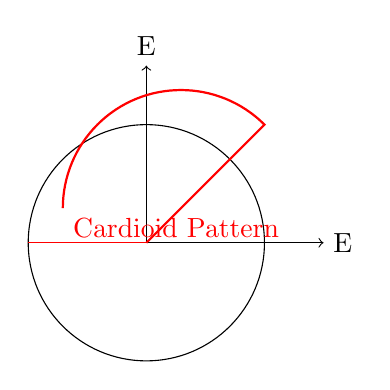
\begin{tikzpicture}[scale=1.5]
    \draw[->] (0,0) -- (1.5,0) node[right] {E};
    \draw[->] (0,0) -- (0,1.5) node[above] {E};
    \draw (0,0) circle(1);
    \draw[thick, red] (0,0) -- (1,1) arc[start angle=45, end angle=180, radius=1]
        node[below right] {Cardioid Pattern};
    \draw[red] (0,0) -- (-1,0);
\end{tikzpicture}
\end{center}

This diagram qualitatively represents the cardioid pattern typical of a single-turn loop antenna, showing the directionally strongest radiation, depicted in red.

In conclusion, the correct answer to the question is \textbf{A: Cardioid}. Understanding these radiation patterns forms a fundamental part of studying antennas, particularly in radio communications and electronics.
